\documentclass[11pt]{article}

% Paquetes
%===================================================================================================

% Establecemos los márgenes
\usepackage[a4paper, margin=1in]{geometry}

% Separacion entre parrafos
\setlength{\parskip}{1em}

% Paquete para incluir codigo
\usepackage{listings}

% Paquete para incluir imagenes
\usepackage{graphicx}
\graphicspath{ {./Imagenes/} }

% Para fijar las imagenes en la posicion deseada
\usepackage{float}

% Para que el codigo acepte caracteres en utf8
\lstset{literate=
  {á}{{\'a}}1 {é}{{\'e}}1 {í}{{\'i}}1 {ó}{{\'o}}1 {ú}{{\'u}}1
  {Á}{{\'A}}1 {É}{{\'E}}1 {Í}{{\'I}}1 {Ó}{{\'O}}1 {Ú}{{\'U}}1
  {à}{{\`a}}1 {è}{{\`e}}1 {ì}{{\`i}}1 {ò}{{\`o}}1 {ù}{{\`u}}1
  {À}{{\`A}}1 {È}{{\'E}}1 {Ì}{{\`I}}1 {Ò}{{\`O}}1 {Ù}{{\`U}}1
  {ä}{{\"a}}1 {ë}{{\"e}}1 {ï}{{\"i}}1 {ö}{{\"o}}1 {ü}{{\"u}}1
  {Ä}{{\"A}}1 {Ë}{{\"E}}1 {Ï}{{\"I}}1 {Ö}{{\"O}}1 {Ü}{{\"U}}1
  {â}{{\^a}}1 {ê}{{\^e}}1 {î}{{\^i}}1 {ô}{{\^o}}1 {û}{{\^u}}1
  {Â}{{\^A}}1 {Ê}{{\^E}}1 {Î}{{\^I}}1 {Ô}{{\^O}}1 {Û}{{\^U}}1
  {ã}{{\~a}}1 {ẽ}{{\~e}}1 {ĩ}{{\~i}}1 {õ}{{\~o}}1 {ũ}{{\~u}}1
  {Ã}{{\~A}}1 {Ẽ}{{\~E}}1 {Ĩ}{{\~I}}1 {Õ}{{\~O}}1 {Ũ}{{\~U}}1
  {œ}{{\oe}}1 {Œ}{{\OE}}1 {æ}{{\ae}}1 {Æ}{{\AE}}1 {ß}{{\ss}}1
  {ű}{{\H{u}}}1 {Ű}{{\H{U}}}1 {ő}{{\H{o}}}1 {Ő}{{\H{O}}}1
  {ç}{{\c c}}1 {Ç}{{\c C}}1 {ø}{{\o}}1 {å}{{\r a}}1 {Å}{{\r A}}1
  {€}{{\euro}}1 {£}{{\pounds}}1 {«}{{\guillemotleft}}1
  {»}{{\guillemotright}}1 {ñ}{{\~n}}1 {Ñ}{{\~N}}1 {¿}{{?`}}1 {¡}{{!`}}1
}

% Para que no se salgan las lineas de codigo
% Para fijar una fuente que resalte
\lstset{breaklines=true, basicstyle=\ttfamily}


% Para que los metadatos que escribe latex esten en español
\usepackage[spanish]{babel}
\decimalpoint % Para que no se cambie el punto a la coma

% Para la bibliografia
% Sin esto, los enlaces de la bibliografia dan un error de compilacion
\usepackage{url}

% Para mostrar graficas de dos imagenes, cada una con su caption, y con un caption comun
\usepackage{subcaption}

% Simbolo de los numeros reales
\usepackage{amssymb}

% Para que los codigos tengan una fuente distinta
\usepackage{courier}

\lstdefinestyle{CustomStyle}{
  language=Python,
  numbers=left,
  stepnumber=1,
  numbersep=10pt,
  tabsize=4,
  showspaces=false,
  showstringspaces=false
  basicstyle=\tiny\ttfamily,
}

% Para incluir tablas en csv
\usepackage{csvsimple}

% Para referenciar secciones usando el nombre de las secciones
\usepackage{nameref}

% Para enumerados dentro de enumerados
\usepackage{enumitem}

% Para mejores tablas
\usepackage{tabularx}

% Para poder tener el mismo identificador en dos tablas separadas
\usepackage{caption}

% Mostrar la página de las referencias en el indice del documento
\usepackage[nottoc,numbib]{tocbibind}

% Para mostrar las matrices
\usepackage{amsmath}

% TODOS:
% [ ] Comentar que solo nos hemos quedado con un conjunto de datos variant1 ??

% Metadatos del documento
%===================================================================================================
\title{
    {Aprendizaje Automático - Proyecto Final}\\
    {\emph{Facebook comment volume prediction}}
}

\author{
    {Sergio Quijano Rey - 72103503k}\\
    {sergioquijano@correo.ugr.es} \\
    {} \\
    {Lucía Salamanca López - 77185623s} \\
    {luciasalamanca@correo.ugr.es}\\
    {} \\
    {4º Doble Grado Ingeniería Informática y Matemáticas}
}

\date{\today}

% Separacion entre parrafos
\setlength{\parskip}{1em}

% Contenido del documento
%===================================================================================================
\begin{document}

% Portada del documento
\maketitle
\pagebreak

% Indice de contenidos
\tableofcontents

% Lista de figuras
\listoffigures

% Lista de tablas
\listoftables

\pagebreak

\section{Identificación del problema}

El problema que hemos escogido para esta práctica final consiste en predecir el número de comentarios que un post en \emph{Facebook} va a recibir horas después de ser publicado. La fuente original de los datos se encuentra en \cite{uci:online}.

En dicha página, se encuentra también la referencia al \emph{paper} original \cite{original_paper:paper}. En dicho paper se comenta el proceso de extracción de los datos, que generan los \emph{datasets} con los que hemos trabajado.

\subsection{Problema a resolver}

Estamos ante un problema de regresión, pues nuestro objetivo es predecir el número de comentarios (variable en principio no finita) a partir de unos datos de entrada. Por tanto, tenemos una función objetivo que viene dada por:

$$f: \mathbb{X} \rightarrow \mathbb{Y}$$

donde $\mathbb{X}$ es el conjunto de las 53 variables aleatorias de entrada, e $\mathbb{Y}$ es la variable aleatoria de salida, entera.

Por lo tanto, nuestro objetivo es encontrar tanto una clase de funciones $\mathcal{H}$ como un algorito de aprendizaje $\mathcal{A}$ que nos devuelva un $h \in \mathcal{H}$ que se asemeje a la función objetivo, es decir

$$h(x) \approx f(x), \forall x \in \mathbb{X}$$

La noción de que ambas funciones sean aproximadas se especificará en \emph{\ref{eleccion_modelos}. \nameref{eleccion_modelos}}.

\subsection{Descripción de las características}

Para obtener las características el autor del paper \cite{original_paper:paper} ha empleado un \emph{crawler} programado en \lstinline{JAVA} y el lenguaje de consulta de \emph{Facebook} (\lstinline{FQL}), con el que se ha recogido información de las páginas de \lstinline{Facebook} de más interés \cite{original_paper:paper}. A partir de dicha informacióm, solo se consideran los comentarios que fueron publicados en los últimos tres días respecto al momento en el que el \emph{crawler} recolecta los datos. Esto pues se presupone que los posts más antiguos no van a recibir más atención. También se eliminan los posts de los que faltan comentarios o algún detalle necesario, de ahí que en nuestro dataset no tengamos \emph{missing values}, como se mostrará en \emph{\ref{exploracion_datos}. \nameref{exploracion_datos}}.

Como se ha dicho previamente tenemmos 53 características que podemos dividirlas en distintos subgrupos.

\subsubsection{Características de la página}

Las extracción de características gira entorno a una de las características principales de \emph{Facebook}, las páginas de \emph{Facebook}. Por tanto, se extraerán características referentes a distintas páginas de \emph{Facebook} con la intención de predecir el número de comentarios que obtendrá un nuevo \emph{post} en dichas páginas.

Existen cuatro características referentes a las páginas:

\begin{itemize}
  \item \textbf{Likes de la página}: describe el apoyo de los usuarios hacia ciertos elementos de dicha página, como comentarios, imágenes, estados, posts\ldots

% TODO -- Esto mejorar
  \item \textbf{Categoría de la página}: define el tipo de entidad o persona sobre la que trata la información tratada en dicha página. El dataset contiene un archivo donde se definen todos los tipos posibles de categorías, como por ejemplo: comercio local, marca comercial, producto, artista, entretenimiento, \ldots

  \item \textbf{\emph{Checkin} de la página}: comprobaciones de actos de presencia en un determinado lugar (sólo es válido para páginas institucionales)

  \item \textbf{\emph{Talking About} de la página}: número de usuarios que vuelven a la página tras darle a like a dicha página. Por volver a la página se entienden actividades como comentar, dar like a un post, compartir un post\ldots
\end{itemize}

\subsubsection{Características esenciales}

En este subgrupo se incluye el comportamiento de los comentarios en el post en distintos intervalos de tiempo respecto a distintas métricas. Se dividen en cinco secciones que dependen de una referencia temporal fijada. El autor fija esta referencia en 72h después de la publicación del \emph{post}.

% TODO -- si da tiempo, hacerlo en una tabla que queda mas profesional
\begin{itemize}
  \item \textbf{C1}: número total de comentarios durante las 72 horas previas a la referencia

  \item \textbf{C2}: número total de comentarios durante las  24 horas previas a la referencia

  \item \textbf{C3}: número total de comentarios entre las 48 y 24 horas previas a la referencia

  \item \textbf{C4}: número total de comentarios en las 24h posteriores a publicar la referencia

  \item \textbf{C5}: diferencia de número total de comentarios entre C2 y C3.

\end{itemize}

A partir de estas características base, calculamos las siguientes estadísticas respecto a los post de una misma página:  mínimo, máximo, media, mediana y desviación típica. Con ello se obtienen 25 características adicionales, que, junto con las cinco características base, conforman 30 características de este subgrupo.

\subsubsection{Características relativas al día de la semana}

Para representar el día de la semana en el que el post fue publicado y el día con respecto a la referencia temporal se usan indicadores binarios. Existen 14 categorías de este tipo.

Se usan 14 características binarias. 7 de ellas para indicar el día de la semana en la que se publicó el post (todas cero salvo el día de publicación). Las otras 7 características indican el día de la semana de la referencia fijada (de nuevo, 72h después de la publicación del post).

\subsubsection{Otras características básicas}

Incluye 5 características tipo medatadatos del post, como puede ser la longitud del post o el número de veces que se ha compartido.

\subsection{Exploración del \emph{Dataset}} \label{exploracion_datos} \label{boxplot}

Como ya hemos comentado, el problema presenta distintas variantes en función de las referencias temporales fijadas. Por tanto, tenemos distintos problemas de regresión con distintos dominios, es decir, no tiene sentido juntar todas las variantes del problema de las que disponemos. Así, nos quedamos solo con los datos relativos a la variante 1.

Con la función \lstinline{explore_dataset}, mostramos algunas estadísticas de las variables aleatorias que componen las columnas de nuestro conjunto de datos. Notar que en esta exploración ya hemos separado el conjunto de \emph{training} y \emph{testing}, con la función \lstinline{split_train_test} que más adelante, en \emph{\ref{preprocesado}. \nameref{preprocesado}}.

Tras esta separación nos quedamos con 32839 ejemplos para entrenamiento y 8210 ejemplos para test.

La descripción de las variables se muestra en la siguiente tabla:

\begin{table}[H]
  \centering
  \resizebox{0.8\columnwidth}{!}{%
  \begin{tabular}{|c|c|c|c|c|c|c|c|c|}
    \hline
    \textbf{col}  &         \textbf{mean}&         \textbf{median}&           \textbf{std}&     \textbf{min}&           \textbf{max}&           \textbf{p25}&           \textbf{p75} \\
    \hline
    0    & 1.32e+6&  292911.00&  7.401e+6&    36.0&  4.86e+8&  37149.00&  1.20e+6 \\
    1    & 4.63e+3&       0.00&  2.045e+4&     0.0&  1.86e+5&      0.00&  9.90e+1 \\
    2    & 4.54e+4&    7237.00&  1.237e+5&     0.0&  6.78e+6&    698.00&  5.14e+4 \\
    3    & 2.42e+1&      18.00&  2.001e+1&     1.0&  1.06e+2&      9.00&  3.20e+1 \\
    4    & 1.46e+0&       0.00&  1.872e+1&     0.0&  2.34e+3&      0.00&  0.00e+0 \\
    5    & 4.42e+2&     235.00&  4.958e+2&     0.0&  2.77e+3&     45.00&  7.17e+2 \\
    6    & 5.53e+1&      23.37&  8.565e+1&     0.0&  2.34e+3&      5.51&  7.18e+1 \\
    7    & 3.53e+1&      12.00&  6.842e+1&     0.0&  2.34e+3&      2.00&  4.20e+1 \\
    8    & 6.72e+1&      35.06&  8.117e+1&     0.0&  1.00e+3&      7.88&  1.02e+2 \\
    9    & 1.62e-1&       0.00&  3.337e+0&     0.0&  3.81e+2&      0.00&  0.00e+0 \\
    10   & 2.84e+2&     118.00&  3.758e+2&     0.0&  2.77e+3&     26.00&  4.01e+2 \\
    11   & 2.21e+1&       8.43&  3.599e+1&     0.0&  9.99e+2&      1.91&  2.90e+1 \\
    12   & 7.42e+0&       2.00&  1.980e+1&     0.0&  7.97e+2&      0.00&  8.00e+0 \\
    13   & 4.04e+1&      17.38&  5.450e+1&     0.0&  8.70e+2&      4.10&  6.07e+1 \\
    14   & 2.90e-2&       0.00&  2.209e+0&     0.0&  3.24e+2&      0.00&  0.00e+0 \\
    15   & 2.67e+2&     116.00&  3.257e+2&     0.0&  1.87e+3&     26.00&  3.81e+2 \\
    16   & 1.95e+1&       8.58&  3.062e+1&     0.0&  4.37e+2&      2.03&  2.48e+1 \\
    17   & 4.87e+0&       1.00&  1.311e+1&     0.0&  4.33e+2&      0.00&  5.00e+0 \\
    18   & 3.85e+1&      18.63&  5.041e+1&     0.0&  5.80e+2&      4.09&  5.38e+1 \\
    19   & 1.38e+0&       0.00&  1.642e+1&     0.0&  1.89e+3&      0.00&  0.00e+0 \\
    20   & 4.14e+2&     224.00&  4.719e+2&     0.0&  2.77e+3&     41.00&  6.70e+2 \\
    21   & 5.23e+1&      21.85&  8.017e+1&     0.0&  1.89e+3&      5.21&  6.83e+1 \\
    22   & 3.37e+1&      12.00&  6.459e+1&     0.0&  1.89e+3&      2.00&  4.00e+1 \\
    23   & 6.29e+1&      32.36&  7.611e+1&     0.0&  8.52e+2&      7.60&  9.62e+1 \\
    24   &-2.19e+2&     -92.00&  2.801e+2& -1677.0&  3.81e+2&   -310.00& -2.10e+1 \\
    25   & 2.75e+2&     109.00&  3.730e+2&  -204.0&  2.77e+3&     23.00&  3.79e+2 \\
    26   & 2.58e+0&       0.27&  1.563e+1&  -210.5&  6.39e+2&     -0.48&  2.97e+0 \\
    27   &-1.99e+0&       0.00&  1.237e+1&  -288.0&  7.97e+2&     -2.00&  0.00e+0 \\
    28   & 5.56e+1&      25.54&  7.372e+1&     0.0&  1.33e+3&      5.99&  8.12e+1 \\
    29   & 5.50e+1&      11.00&  1.345e+2&     0.0&  2.34e+3&      2.00&  4.60e+1 \\
    30   & 2.20e+1&       2.00&  7.666e+1&     0.0&  2.09e+3&      0.00&  1.20e+1 \\
    31   & 1.94e+1&       0.00&  6.916e+1&     0.0&  1.59e+3&      0.00&  9.00e+0 \\
    32   & 5.20e+1&      10.00&  1.258e+2&     0.0&  2.18e+3&      2.00&  4.40e+1 \\
    33   & 2.64e+0&       0.00&  9.292e+1& -1277.0&  2.09e+3&     -6.00&  3.00e+0 \\
    34   & 3.51e+1&      35.00&  2.099e+1&     0.0&  7.20e+1&     17.00&  5.30e+1 \\
    35   & 1.64e+2&      97.00&  3.826e+2&     0.0&  2.14e+4&     38.00&  1.72e+2 \\
    36   & 1.17e+2&      13.00&  1.023e+3&     1.0&  1.44e+5&      2.00&  6.00e+1 \\
    37   & 0.00e+0&       0.00&  0.000e+0&     0.0&  0.00e+0&      0.00&  0.00e+0 \\
    38   & 2.37e+1&      24.00&  2.008e+0&     1.0&  2.40e+1&     24.00&  2.40e+1 \\
    39   & 1.22e-1&       0.00&  3.273e-1&     0.0&  1.00e+0&      0.00&  0.00e+0 \\
    40   & 1.43e-1&       0.00&  3.506e-1&     0.0&  1.00e+0&      0.00&  0.00e+0 \\
    41   & 1.49e-1&       0.00&  3.566e-1&     0.0&  1.00e+0&      0.00&  0.00e+0 \\
    42   & 1.56e-1&       0.00&  3.622e-1&     0.0&  1.00e+0&      0.00&  0.00e+0 \\
    43   & 1.45e-1&       0.00&  3.525e-1&     0.0&  1.00e+0&      0.00&  0.00e+0 \\
    44   & 1.45e-1&       0.00&  3.523e-1&     0.0&  1.00e+0&      0.00&  0.00e+0 \\
    45   & 1.37e-1&       0.00&  3.443e-1&     0.0&  1.00e+0&      0.00&  0.00e+0 \\
    46   & 1.43e-1&       0.00&  3.502e-1&     0.0&  1.00e+0&      0.00&  0.00e+0 \\
    47   & 1.31e-1&       0.00&  3.382e-1&     0.0&  1.00e+0&      0.00&  0.00e+0 \\
    48   & 1.37e-1&       0.00&  3.443e-1&     0.0&  1.00e+0&      0.00&  0.00e+0 \\
    49   & 1.50e-1&       0.00&  3.572e-1&     0.0&  1.00e+0&      0.00&  0.00e+0 \\
    50   & 1.49e-1&       0.00&  3.564e-1&     0.0&  1.00e+0&      0.00&  0.00e+0 \\
    51   & 1.44e-1&       0.00&  3.518e-1&     0.0&  1.00e+0&      0.00&  0.00e+0 \\
    52   & 1.44e-1&       0.00&  3.514e-1&     0.0&  1.00e+0&      0.00&  0.00e+0 \\
    53   & 7.43e+0&       0.00&  3.588e+1&     0.0&  1.30e+3&      0.00&  3.00e+0 \\
    \hline
  \end{tabular}
}
\caption{Exploración estadística de los atributos del conjunto de entrenamiento}
\end{table}

En la tabla no hemos mostrado la estadística de \emph{missing values}, pues como ya hemos comentado, no tenemos datos faltantes en este \emph{dataset}. Tampoco mostramos la columna en la que se muestra el tipo, pues todas las variables son o bien flotantes o bien enteras, y por tanto no es necesaria una técnica de codificación de variables categóricas como puede ser \emph{one hot encoding}.

En esta tabla queda clara la necesidad de realizar un proceso de estandarización o bien de normalización. Los modelos que vamos a emplear son muy sensibles a variables en escalas diferentes. Otros directamente se comportam mucho mejor cuando tenemos media cero y desviación típica uno.

Estas escalas diferentes se pueden ver, por ejemplo, con la columna 0 que se mueve en el rango $[36.0, 4.86 * 10^8]$ y que tiene una desviación típica de $7.4 * 10^6$, mientras que la columna 43 se mueve en el rango $[0, 1]$ y tiene una desviación típica de $3.5 * 10$.

En la función \lstinline{explore_dataset} también hacemos un gráfico de cajas y bigotes de la variable de salida, obteniendo la siguiente gráfica:

\begin{figure}[H]
  \centering
  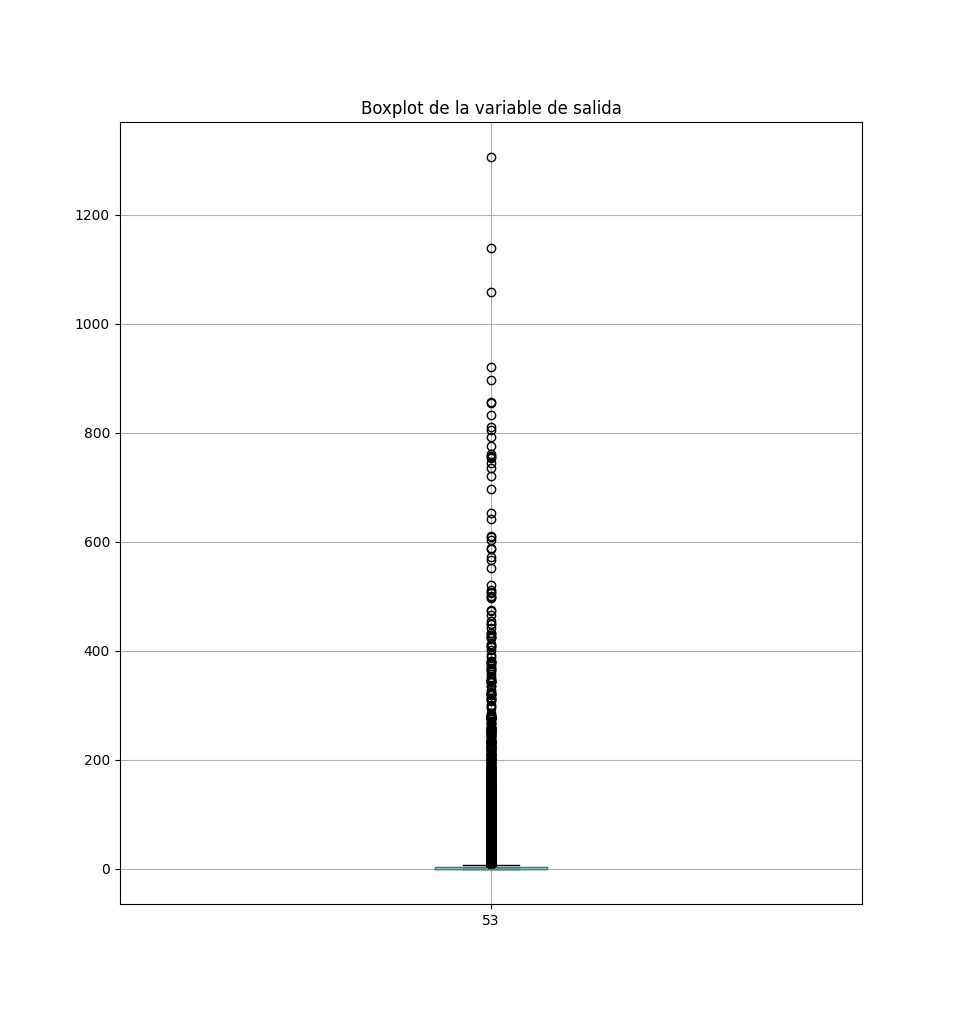
\includegraphics[width=0.5\textwidth]{boxplot_salida}
  \caption{Gráfico de cajas y bigotes de la variable de salida}
\end{figure}

Por la cantida de valores atípicos, no se ve bien que sea una gráfica de cajas y bigotes, así que hacemos \emph{zoom} en la imagen obteniendo la siguiente gráfica:

\begin{figure}[H]
  \centering
  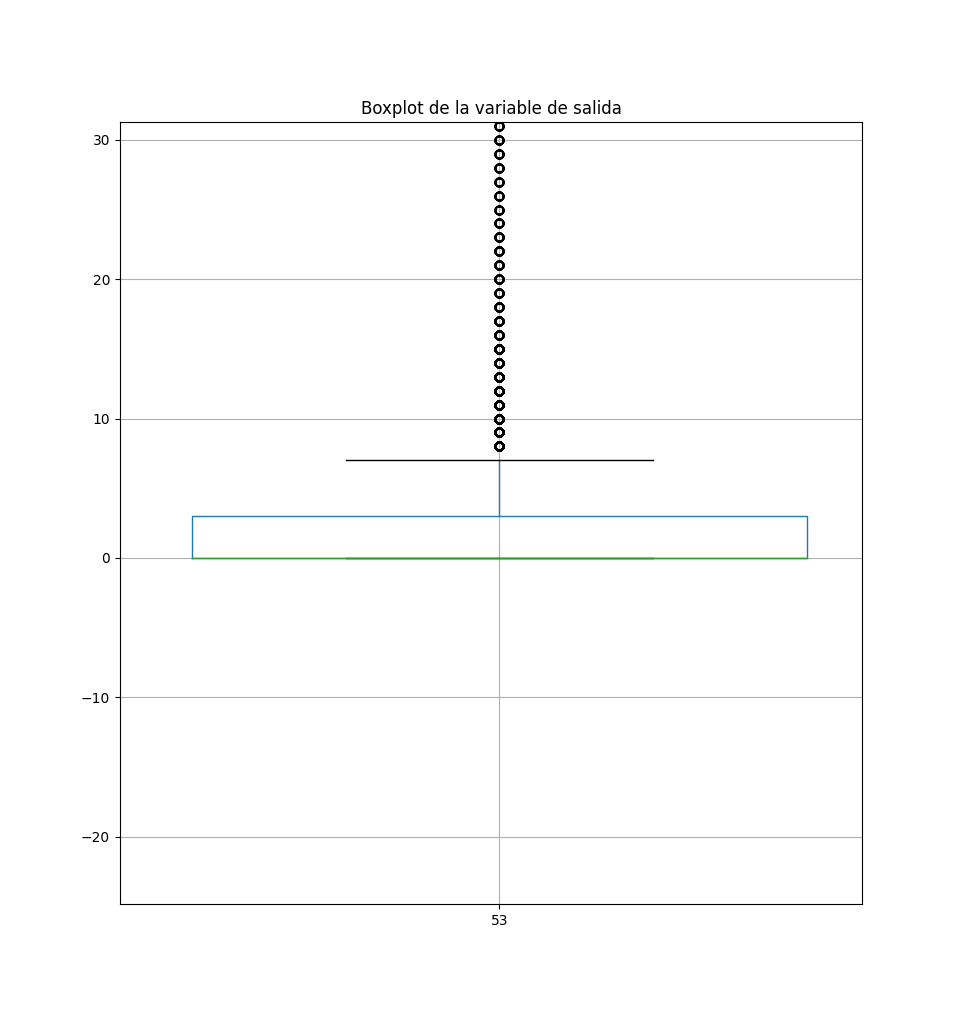
\includegraphics[width=0.5\textwidth]{boxplot_salida_zoom}
  \caption{Gráfico de cajas y bigotes de la variable de salida, \textbf{ampliada}}
\end{figure}

A partir de estas gráficas quedan claros los siguientes hechos:

\begin{itemize}
  \item Todos los elementos que quedan por debajo del percentil 75 en la variable de salida tienen menos de 10 comentarios.
  \item El rango intercuartílico es muy pequeño, por tanto, sabemos que los datos, en su variable de salida, están muy concentrados en un número de comentarios muy bajo
  \item Tenemos una gran cantidad de valores atípicos en la variable de salida. Atípicos en el sentido de que se alejan del percentil 75 más de 1.5 veces el rango intercuartílico
\end{itemize}

Por tanto, como se comentará en \emph{\ref{metrica_error}. \nameref{metrica_error}}, es una buena idea escoger como métrica de error para nuestros modelos el error cuadrático medio, pues penaliza más predicciones que se alejen de los valores de etiquetado. Con ello intentamos evitar que los modelos tiendan a predecir constantemente un valor bajo de comentarios, pues la mayoría de los datos están concentrados en este rango de salida.
\pagebreak

\section{Preprocesamiento de los datos} \label{preprocesado}

El preprocesamiento de los datos se divide en tres etapas: estandarización, selección de componentes principales y transformación polinómica de los datos.

A la hora de aplicar \emph{Cross Validation} para seleccionar nuestro modelo final, compararemos los resultados obtenidos tanto en el conjunto transformado con \emph{PCA} y trasnformaciones polinómicas como en el conjunto de datos original al que solo hemos aplicado estandarización, quedándonos con el conjunto de datos en el que se haya encontrado la hipótesis con mejores resultados.

\subsection{Eliminación de outliers}

A la hora de borrar \emph{outliers} no hemos seguido la técnica básica de eliminar aquellos ejemplos en los que, en alguna variable aleatoria, se alejen de la media más de tres veces la desviación típica. Esta aproximación univariante eliminaba un porcentaje demasiado alto de los datos, y por tanto, hemos decidido emplear una técnica más inteligente a la hora de borrar los valores atípicos, basada en la distancia de Mahalanobis. Esta distancia se parece a la distancia euclíde, sin embargo, se tiene en cuenta la correlación entre las variables aleatorias \cite{wiki_mahalanobis:online}.

Para eliminar los outliers hacemos uso de la función \lstinline{remove_outliers} que a su vez, hace uso de la función proporcionada por \emph{sklearn} \lstinline{EllipticEnvelope}. En esta técnica estamos suponiendo que nuestro \emph{dataset} sigue aproximadamente una distribución Gaussiana multidimensional. Intenta ajustar una elipse a los puntos centrales, ignorando los puntos que quedan fuera de esta elipse ajustada. La distancia de Mahalanobis se usa como una medida de cómo de atípico es un punto de nuestro \emph{dataset} \cite{sklearn_outlier:online}. Esta distancia viene dada por.

$$d_m(x, y) := \sqrt{(x - y)^T \Sigma^{-1} (x - y)}$$

Es importante comentar el uso del parámetro \lstinline{contamination}. Este parámetro indica la proporción de \emph{outliers} que estimamos que tiene nuestro \emph{dataset}, es decir, la \emph{"contaminación"} esperada del \emph{dataset}. En nuestro caso hemos fijado este valor a un $5\%$.

Es importante realizar como primer paso el borrado de \emph{outliers}, pues las posteriores técnicas como estandarización o análisis de componentes principales son muy sensibles a estos \emph{outliers}.

\subsection{Estandarización de los datos}

A la hora de estandarizar los datos, buscamos que las variables aleatorias de nuestro \emph{dataset} sigan una distribución normal de media cero y desviación típica uno.

Para ello, y supuesta la hipótesis de que nuestras variables siguen una distribución normal de media y varianza desconocida, usamos el hecho de que cualquier variable aleatoria $X$ que siga una normal verifica que:
$$X_{norm} := \frac{{X- \bar{X}}}{X_{\sigma}} \Longrightarrow X_{norm} \sim \mathcal{N}(0, 1)$$

La media y la desviación típica son muy sensibles a valores atípicos, por lo que es necesario quitar los \emph{outliers} antes de estandarizar nuestros datos, como ya hemos comentado.

Tras dicha limpieza de outliers aplicamos el estandarizado con la función \lstinline{standarize_dataset}, que hace uso de la función \lstinline{StandardScaler} proporcionada por \emph{sklearn}.

A esta función le pasamos como parámetros tanto el conjunto de entrenamiento como el conjunto de test. El conjunto de test no se usa a la hora de calcular la transformación, solo se emplea el conjunto de entrenamiento para estos cálculos. El conjunto de test se pasa con el único propósito de aplicar la misma trasnformación que la calculada y aplicada en el conjunto de test. Todo esto para no caer en un caso de \emph{data snooping}.

Como hemos comentado previamente, todos los datos con los que vamos a entrenar los distintos modelos van a pasar por estas dos primeras etapas, por lo que, tras haber eliminado los \emph{outliers} y haber estandarizado nuestros datos, haremos una copia de nuestros datos en \lstinline{df_train_original_x} y \lstinline{df_test_original_x}.

Tras estandarizar los datos, mostramos las estadísticas de algunas columnas del conjunto estandarizado:

\begin{table}[H]
  \centering
  \begin{tabular}{|c|c|c|c|c|c|c|c|c|}
  \hline
\textbf{col}  &         \textbf{mean}&         \textbf{median}&           \textbf{std}&     \textbf{min}&           \textbf{max}&           \textbf{p25}&           \textbf{p75} \\
\hline
0  &  3.250e-17& -0.34&  1.00&  -0.47&   15.65& -0.45& -0.00\\
1  &  7.671e-16& -0.22&  1.00&  -0.22&    9.02& -0.22& -0.22\\
2  & -1.947e-16& -0.46&  1.00&  -0.56&    9.33& -0.55&  0.17\\
3  &  1.025e-15& -0.32&  1.00&  -1.17&    4.02& -0.77&  0.36\\
\ldots  &  \ldots & \ldots &  \ldots &  \ldots &    \ldots & \ldots &  \ldots \\
50 &  1.250e-16& -0.41&  1.00&  -0.41&    2.40& -0.41& -0.41\\
51 &  4.213e-16& -0.41&  1.00&  -0.41&    2.43& -0.41& -0.41\\
52 & -7.532e-16& -0.41&  1.00&  -0.41&    2.43& -0.41& -0.41\\
\hline
  \end{tabular}
  \caption{Estadísticas del \emph{dataset} tras estandarizar}
  \label{tabla_std}
\end{table}

Nuestro proceso de estandarización en principio solo se preocupa de conseguir media cero y desviación típica uno. Pero como se puede apreciar en la anterior tabla, este proceso provoca colateralmente que el rango de las distintas variables no sea tan dispar, lo cual es beneficioso como ya se ha comentado.

\subsection{Análisis de Componentes Principales (PCA)}

Para el análisis de componentes principales hacemos uso de la función \lstinline{apply_PCA}. Queremos que tras la transformación de nuestro espacio obtengamos el $99\%$ de la varianza de nuestro \emph{dataset} original. Por tanto, pasaremos a la función \lstinline{PCA} de \emph{sklearn} el parámetro \lstinline{n_components} igualado a $0.99$, lo que fuerza a que seleccione el número de componentes principales necesarias para explicar el $99\%$ o más de nuestra varianza.

% TODO -- explica mejor esto chiquilla
Vamos a observar en la siguiente tabla el número de componentes que obtenemos con el $99\%$ de la varianza y la varianza explicada en cada una de ellas. El método de \emph{PCA} devuelve las componentes ordenadas de mayor varianza explicada a menor.

% TODO -- poner solo 3 cifras decimales que Nicolas lo penaliza
\begin{table}[!htb]
  \begin{tabular}{|c|c|}
    \hline
    \textbf{Nº de componente}  &         \textbf{Varianza explicada} \\
    \hline
    1& 0.365 \\
    2& 0.044\\
    3& 0.040\\
    4& 0.039\\
    5& 0.038\\
    6& 0.037\\
    7& 0.032\\
    8& 0.026\\
    9& 0.025 \\
    10& 0.024\\
    11& 0.023\\
    12& 0.021\\
    13& 0.021\\
    14& 0.020\\
    15& 0.020\\
    16& 0.020\\
    \hline
  \end{tabular}
  \quad
  \begin{tabular}{|c|c|}
    \hline
    \textbf{Nº de componente}  &         \textbf{Varianza explicada} \\
    \hline
    17& 0.019\\
    18& 0.019\\
    19& 0.018\\
    20& 0.017\\
    21& 0.016\\
    22& 0.016\\
    23& 0.016\\
    24& 0.014\\
    25& 0.012\\
    26& 0.007\\
    27& 0.007\\
    28& 0.006\\
    29& 0.006\\
    30& 0.005\\
    31& 0.003\\
    \hline
  \end{tabular}
\caption{Varianza explicada por las componentes principales obtenidas}
\end{table}

Tenemos un total de 31 componentes que explican el 0.9906 de la varianza. Obtenemos así que la dimensionalidad de nuestro espacio muestral se reduce un $40\%$ aproximadamente.

Tras aplicar \emph{PCA}, las variables vuelven a estar en rangos dispares. Sin embargo, esperamos a aplicar las trasnformaciones no lineales de los datos para volver a realizar la estandarización.

\subsection{Transformación polinómica}

% TODO -- hablar de d_vc

Al haber reducido la dimensionalidad de nuestro espacio, el tamaño de nuestro \emph{dataset} permite realizar una transformación cuadrática de nuestros datos sin que el coste computacional sea excesivo, y sin que tengamos problemas de generalización.

Hemos considerado esta transformación pues no disponemos de conocimiento experto del problema para decidir en base a ello una tal transformación. Tampoco en el \emph{paper} original \cite{original_paper:paper} se presenta una transformación en base a conocimiento experto.

Por tanto, consideramos una transformación polinómica $\phi_q$ de grado $q$ fijado, pues pueden dar buenos resultados sin mucha información a priori. Fijamos $q=2$ por el coste computacional ya mencionado y por buscar una buena generalización. Una transformación polinómica de mayor grado no sería abordable en nuestras máquinas (hicimos la prueba y comprobamos que, efectivamente, no era abordable en un tiempo razonable) y podría llegar a dar problemas de generalización.

% TODO - la frase de los monomios es que la dices mejor y me he enterado regular
La transformación consiste en considerar los monomios en varias variables de hasta grado 2. Por ejemplo, $x_1 x_2, x_1, x_1^2, \ldots$

La dimensión de nuestro espacio transformado es entonces

$$d = {1+2n}+{{n(n-1)}\over{2}} = {1+2*31}+{{31*30}\over{2}} = 528$$

donde $n$ es el tamaño de nuestro conjunto de entrenamiento.

Ahora, tenemos varianzas y rangos de las variables dispares. Esto es claro porque estamos considerando transformaciones no lineales que no van a respetar las escalas similares de nuestros datos, ni la distribución centrada en cero. Por tanto es necesario aplicar de nuevo estandarización al nuevo conjunto de entrenamiento. El efecto es el mismo que el comentado en la \emph{Tabla \ref{tabla_std}. \nameref{tabla_std}}, y por tanto no mostramos esta tabla ya que no va a aportar información nueva.

\pagebreak

\section{Selección del modelo} \label{seleccion_modelos} \label{metrica_error}

Vamos a emplear la técnica \emph{k-fold Cross Validation} para elegir la mejor hipótesis entre distintas clases de funciones. Además, usaremos esta técnica para decidir si usamos el conjunto original de los datos a los que solo aplicamos estandarización, o si bien usamos el conjunto al que aplicamos \emph{PCA} y polinomios de grado dos.

En todos los modelos que consideramos, consideramos como métrica de evaluación el error cuadrático medio. En regresión hemos visto pocas alternativas, algunas como el error absoluto medio o el coeficiente R2. Sin embargo, consideramos el error cuadrático medio pues todos los modelos considerados usan esta métrica como métrica de error a minimizar, y es una métrica fácilmente interpretable.

Además, como ya se ha comentado, la distribución de los datos de salida hace que sea más deseable esta métrica de error, para evitar que el modelo tienda a predecir constantemente valores bajos.

\subsection{Modelos Candidatos}

\subsubsection{Regresión lineal} \label{regresion_lineal}

Para los modelos lineales vamos a considerar el ajuste de un hiperplano usando dos tipos de regularización: Ridge y Lasso.

El interés de estos modelos lineales es que suponen usar modelos de baja complejidad, que probablemente no tengan apenas problemas de generalización, y que a pesar de su sencillez funcionan bien en muchos casos.

Podríamos haber fijado un tipo de regularización en base al problema con el que estamos tratando. Sin embargo, como estamos comparando dos conjuntos de datos distintos, probamos con los dos regularizadores. En el modelo al que aplicamos \emph{PCA} y las transformaciones polinómicas nos decantamos por emplear \emph{Lasso}, pues fuerza a que algunas componentes sean cero, y esto es interesante para anular términos de la transformación polinómica que no sean interesantes. En el conjunto de datos original, tenemos 52 características para un total de 32839 ejemplos de entrenamiento. Usando la regla práctica vista en teoría $N >> d_{VC} * 10$, y teniendo en cuenta que en el caso de 52 variables y que estamos considerando modelos lineales, se verifica con mucho márgen que $32839 >> 10 * 53$. Es por esto que probamos con Ridge, no tenemos la necesidad a priori de ignorar algunas características.

Para Ridge usamos el clasificador \lstinline{Ridge} y para Lasso el clasificador \lstinline{Lasso}, ambos de la librería \lstinline{sklearn}. Los parámetros prefijados son:

\begin{itemize}
  \item \textbf{Máximo de iteraciones}: 10.000
  \item \textbf{Tolerancia}: $10^{-4}$
  \item \textbf{Resolutor para Ridge}: Cholesky
\end{itemize}

Estamos fijando \emph{Cholesky} como resolutor para \emph{Ridge}. De la documentación oficial de \lstinline{sklearn} \cite{sk_linear:online}, sabemoss que  esste resolutor usa una solución cerrada usando el despeje matricial proporcionado por \lstinline{scipy.linalg.solve}. Para \emph{Lasso}, se usa \emph{Coordinate Descent} como algoritmo de aprendizaje. En este algoritmo, en cada paso, se escoge una coordenada según una política dada, y se minimiza variando esa coordenada, dejando el resto fijas \cite{coordinate_descent:online}.

Los parámetros que probamos con \emph{Cross Validation} son:

\begin{itemize}
  \item \textbf{Alpha} (constante de regularización): $\alpha \in \{0.1, 1, 2\}$
\end{itemize}

\subsubsection{\emph{MLP} con tres capas} \label{mlp}

Consideramos \emph{MLP} por su gran expresividad y potencia. Debemos tener cuidado porque estos modelos tienen mucha facilidad de caer en el sobreajuste. Por ese motivo, fijamos algunas medidas de regularización para evitar que esto pase.

Hacemos uso del clasificador \lstinline{MLPRegressor} de \emph{sklearn}. Los parámetros prefijados son:

\begin{itemize}
  \item \textbf{Resolutor}: Adam
  \item \textbf{Tasa de aprendizaje}: 0.001
  \item \textbf{Tolerancia}: $10^-4$
  \item Usamos \textbf{\emph{Early Stopping}} como medida de regularización
  \item \textbf{Función de activación}: ReLU $f(x) := \max{0,x}$
\end{itemize}

No consideramos la función de activación $tanh$ porque esta es más adecuada para problemas de clasificación. Usamos la función \emph{Rectified Linear Activation Unit} en vez de la función sigmoide porque son menos fáciles de saturar en el entrenamiento, implican cómputos más sencillos y no sufren del problema del desvanecimiento del gradiente \cite{relu:online}.

Además, usamos como algoritmo de aprendizaje \emph{Adam}. Es una extensión del algoritmo \emph{SGD}.

En \emph{SGD} mantenemos un \emph{learning rate} fijo durante todo el entrenamiento. En \emph{Adam} se usa el primer y segundo momento del gradiente para variar el \emph{learning rate}, usando una media exponencial sobre estos dos elementos en la que se pueden fijar los parámetros para controlar el decaimiento \cite{adam:online}.

Como ventajas que nos llevan a emplear este algoritmo, podemos citar que es computacionalmente eficiente, apropiado para problemas con muchos datos o altas dimensionalidades, poco afectado por gradientes dispersos o con mucho rudio. Su eficacia ha sido probada en distintos casos de uso reales.

Los parámetros que probamos con \emph{Cross Validation} son:

\begin{itemize}
  \item \textbf{Número de neuronas por capa}: 50, 75 y 100
  \item \textbf{Alpha} (constante de regularización): $\alpha \in \{0.01, 0.1, 1\}$
  \item \textbf{Tipo de regularización}: Ridge
\end{itemize}

Por tanto, estamos usando regularización \emph{Ridge} y \emph{early stopping} como dos medidas de regularización, porque como ya hemos comentado, estos modelos tienen mucha facilidad de sobreajustarse a los datos de entrenamiento.

\subsubsection{Random Forest} \label{random_forest}

Hacemos uso del clasificador \lstinline{RandomForestRegressor} de \emph{sklearn}. De nuevo, este modelo tiene mucha capacidad de sobreajuste, y por tanto, será necesario establecer medidas de regularización para evitar que esto pase.

Este modelo, gracias al empleo de \emph{Bagging} y que se usan árboles no correlados, es muy robusto y eficiente.

Los parámetros prefijados son:

\begin{itemize}
  \item \textbf{Criterio de evaluación}: MSE
  \item Usamos \textbf{bootstraping}.
  \item \textbf{Máximo de características}: fijamos el número de características usadas para la elección del mejor split a la raíz cuadrada del número total de características.
\end{itemize}

Los parámetros que probamos con \emph{Cross Validation} son:

\begin{itemize}
  \item \textbf{Número de árboles}: 90, 95, 100 y 120
  \item \textbf{Profundidad máxima del árbol}: 50 y 100
  \item Número mínimo de muestras necesarias por cada \textbf{nodo hoja}: 2 y 3
\end{itemize}

Usamos la profundidad máxima del árbol y el número mínimo de ejemplos en las hojas como medida de regularización. A menor profundidad mayor intensidad de regularización. Y a mayor número mínimo de ejemplos en las hojas mayor intensidad de regularización. Con estas dos medidas buscamos evitar que el modelo fácilmente sobreajuste los datos.

Como el algoritmo de aprendizaje se usa el algoritmo \emph{greedy} que se ha explicado en las transparencias de teoría aplicado a cada uno de los $n$ árboles.

\subsection{Resultados de \emph{Cross Validation}} \label{cross_validation}

El código que lanza \emph{Cross validation} se encuentra en la función \lstinline{show_cross_validation}.

Esta función hace uso de \emph{GridSearchCV} de \emph{sklearn}. Mediante el uso del parámetro \lstinline{scoring} indicamos que queremos usar el error cuadrático medio cambiado de signo como error de validación.

\lstinline{sklearn} devuelve las métricas de error en negativo. Estas métricas de error se usan en otros módulos de \lstinline{sklearn} donde se busca resolver un problema de maximización. Como se busca minimizar el error, se cambia el signo a este para pasar a un problema de maximización.

Esta función está comentada en el código, pues supone un tiempo demasiado largo de cómputo. En nuestra máquina tarda aproximadamente 4 horas \footnote{Ver en \emph{\ref{apendice}. \nameref{apendice}} las características de la máquina que se ha usado para la ejecución}, mientras que en \emph{Google Colab}, usando el plan gratuito, tarda una hora y media aproximadamente.

Los resultados obtenidos se muestran en las siguientes tablas:

\subsubsection{Resultados sobre el conjunto de datos sin aplicar PCA}

% TODO -- Sin PCA
\begin{table}[H]
  \centering
  \begin{tabular}{|c|c|c|c|}
  \hline
    \textbf{Regularizador} & \textbf{Alpha} & \textbf{Media MSE} & \textbf{STD MSE} \\
    \hline
    Lasso & 0.1 &  -433.93 & 129.83 \\
    Lasso & 1.0 &  -438.05 & 132.39 \\
    Lasso & 2.0 &  -447.14 & 135.17 \\
    Ridge & 0.1 & -432.32  & 122.47  \\
    \textbf{Ridge} & \textbf{1.0}    & \textbf{-432.31}& \textbf{122.33}  \\
    Ridge & 2.0  & -432.33 & 122.25  \\
    \hline
  \end{tabular}
  \caption{Resultados de \emph{Cross Validation} en el \textbf{modelo lineal}}
\end{table}


\begin{table}[H]
  \centering
  \begin{tabular}{|c|c|c|c|}
  \hline

\textbf{Alpha} & \textbf{Nº Neuronas Capas Ocultas} & \textbf{Media MSE} & \textbf{STD MSE} \\
\hline
0.01 & 50   & -323.81  & 201.35  \\
0.01 & 75   & -319.83  & 173.27  \\
0.01 & 100  & -319.07  & 175.99  \\
0.1  & 50   & -325.27  & 176.11  \\
0.1  & 75   & -324.87  & 169.28  \\
0.1  & 100  & -323.01  & 191.74  \\
1    & 50   & -323.84  & 180.41  \\
1    & 75   & -317.44  & 183.94  \\
\textbf{1}    & \textbf{100}  & \textbf{-316.19}  & \textbf{181.75}  \\
\hline
  \end{tabular}
  \caption{Resultados de \emph{Cross Validation} en \textbf{MLP}}
\end{table}
% ======================
\begin{table}[H]
  \centering
  \resizebox{\columnwidth}{!}{%
  \begin{tabular}{|c|c|c|c|c|}
  \hline
  \textbf{Profundidad} & \textbf{Mínimo de ejemplos en los nodos} & \textbf{Nº Estimadores} & \textbf{Media MSE} & \textbf{STD MSE} \\
\hline
5   & 2 & 90    & -332.26 & 155.68 \\
5   & 2 & 95    & -335.48 & 158.10 \\
5   & 2 & 100   & -336.01 & 159.47 \\
5   & 2 & 120   & -332.48 & 158.83 \\
5   & 3 & 90    & -334.00 & 157.50 \\
5   & 3 & 95    & -331.92 & 157.71 \\
5   & 3 & 100   & -330.62 & 160.39 \\
5   & 3 & 120   & -333.84 & 158.25 \\
\textbf{10}  & \textbf{2} & \textbf{90}    & \textbf{-273.66} & \textbf{139.67} \\
10  & 2 & 95    & -274.06 & 138.53 \\
10  & 2 & 100   & -277.89 & 139.97 \\
10  & 2 & 120   & -275.36 & 139.87 \\
10  & 3 & 90    & -275.87 & 142.19 \\
10  & 3 & 95    & -276.18 & 142.63 \\
10  & 3 & 100   & -276.44 & 140.24 \\
10  & 3 & 120   & -279.28 & 142.70 \\
\hline
  \end{tabular}}
  \caption{Resultados de \emph{Cross Validation} en \textbf{RandomForest}}
\end{table}

\begin{table}[H]
  \centering
  \resizebox{\columnwidth}{!}{
  \begin{tabular}{|c|c|c|c|}
  \hline
  \textbf{Modelo} & \textbf{Parametros} & \textbf{Media MSE} & \textbf{STD MSE} \\
  \hline
  Ridge  & $\alpha$ = 1  & -432.31 & 122.33  \\
  MLP    & $\alpha$ = 1, nº neur = 100 & -316.19  & 181.75 \\
  \textbf{RandomForest} & profundidad = \textbf{10}, min ejemplos = \textbf{2} nº estimadores = \textbf{90} & \textbf{-273.66} & \textbf{139.67} \\
\hline
  \end{tabular}}
  \caption{Mejores resultados}
\end{table}

A vista de estos resultados, vemos que en el conjunto de entrenamiento sin aplicar \emph{PCA}, el mejor algoritmo ha sido \emph{Random Forest} con sus mejores parámetros. Sin embargo, los mejores parámetros para \emph{Ridge} logran un modelo más estable que \emph{Random Forest}, como muestra la desviación típica del \emph{MSE} entre los 10 \emph{folds} empleados.

Además, se confirma nuestra hipótesis de que, en este \emph{dataset} con pocas columnas, iba a funcionar mejor el regularizador \emph{Ridge}.

\subsubsection{Resultados sobre el conjunto de datos al que hemos aplicado \emph{PCA} y transformaciones polinómicas}

\begin{table}[H]
  \centering
  \begin{tabular}{|c|c|c|c|}
  \hline
    \textbf{Regularizador} & \textbf{Alpha} & \textbf{Media MSE} & \textbf{STD MSE} \\
    \hline
    \textbf{Lasso} & \textbf{0.1} & \textbf{-369.36} & \textbf{117.27}  \\
    Lasso & 1.0 & -422.36 & 126.32  \\
    Lasso & 2.0 & -463.91 & 133.16  \\
    Ridge & 0.1 & -114052.07 & 320694.41 \\
    Ridge & 1.0 & -2634.53   &   5722.91 \\
    Ridge & 2.0 & -1049.48   &   1699.59 \\
    \hline
  \end{tabular}
  \caption{Resultados de \emph{Cross Validation} en el \textbf{modelo lineal}}
\end{table}

\begin{table}[H]
  \centering
  \begin{tabular}{|c|c|c|c|}
  \hline

\textbf{Alpha} & \textbf{Nº Neuronas Capas Ocultas} & \textbf{Media MSE} & \textbf{STD MSE} \\
\hline
0.01 & 50   & -374.04 & 178.41 \\
0.01 & 75   & -354.91 & 181.29 \\
0.01 & 100  & -355.76 & 186.29 \\
0.1  & 50   & -355.13 & 174.81 \\
0.1  & 75   & -381.34 & 159.67 \\
0.1  & 100  & -367.31 & 177.25 \\
1    & 50   & -353.95 & 168.25 \\
\textbf{1}    & \textbf{75}   & \textbf{-348.79} & \textbf{171.30} \\
1    & 100  & -357.69 & 180.35 \\
\hline
  \end{tabular}
  \caption{Resultados de \emph{Cross Validation} en \textbf{MLP}}
\end{table}

\begin{table}[H]
  \centering
  \resizebox{\columnwidth}{!}{%
  \begin{tabular}{|c|c|c|c|c|}
  \hline
  \textbf{Profundidad} & \textbf{Mínimo de ejemplos en los nodos} & \textbf{Nº Estimadores} & \textbf{Media MSE} & \textbf{STD MSE} \\
\hline
5   & 2 & 90    & -445.43 & 171.04 \\
5   & 2 & 95    & -448.79 & 174.59 \\
5   & 2 & 100   & -447.15 & 174.10 \\
5   & 2 & 120   & -447.23 & 172.69 \\
5   & 3 & 90    & -445.92 & 176.28 \\
5   & 3 & 95    & -446.91 & 175.16 \\
5   & 3 & 100   & -445.29 & 173.27 \\
5   & 3 & 120   & -444.10 & 174.23 \\
10  & 2 & 90    & -408.38 & 165.83 \\
10  & 2 & 95    & -411.08 & 166.98 \\
10  & 2 & 100   & -409.90 & 164.27 \\
10  & 2 & 120   & -408.67 & 165.90 \\
10  & 3 & 90    & -406.30 & 164.12 \\
10  & 3 & 95    & -405.95 & 165.13 \\
\textbf{10}  & \textbf{3} & \textbf{100}   & \textbf{-405.88} & \textbf{164.58} \\
10  & 3 & 120   & -406.93 & 165.64 \\
\hline
  \end{tabular}}
  \caption{Resultados de \emph{Cross Validation} en \textbf{RandomForest}}
\end{table}

\begin{table}[H]
  \centering
  \resizebox{\columnwidth}{!}{
  \begin{tabular}{|c|c|c|c|}
  \hline
  \textbf{Modelo} & \textbf{Parametros} & \textbf{Media MSE} & \textbf{STD MSE} \\
  \hline
  Lasso  & $\alpha$ = 0.1  & -369.36 & 117.27  \\
  \textbf{MLP}    & $\alpha$ = \textbf{1}, nº neur = \textbf{75} & \textbf{-348.79}  & \textbf{171.30} \\
  RandomForest & profundidad = 10, min ejemplos = 3 nº estimadores = 100 & -405.88 & 164.58 \\
\hline
  \end{tabular}}
  \caption{Mejores resultados}
\end{table}

\pagebreak

\section{Selección del modelo final}

\subsection{Entrenamiento sobre todo el conjunto de entrenamiento}

Tras haber aplicado \emph{Cross Validation}, obtenemos que el modelo óptimo es \emph{Random Forest} con parámetros:

\begin{itemize}
  \item Profundidad: 10
  \item Número mínimo de ejemplos en las hojas: 2
  \item Número de árboles estimadores: 90
  \item Conjunto de datos: \emph{training set} original al que solo aplicamos borrado de \emph{outliers} y  estandarización
\end{itemize}

\subsection{Resultados obtenidos}

Una vez entrenado sobre todo el conjunto de entrenamiento, mostramos los resultados con las funciones \lstinline{show_results} y \lstinline{learning_curve}. Los resultados de la primera función se resumen en la siguiente tabla:

\begin{table}[H]
    \centering
    \begin{tabular}{|c|c|c|c|}
    \hline
    \textbf{Conjunto de datos}  & \textbf{MSE} & \textbf{MAE} & \textbf{$R^2$} \\
    \hline
    Training & 131.28  & 2.68 & 0.77 \\
    Testing  & 541.50  & 4.81 & 0.55 \\
    \hline
    \end{tabular}
    \caption{Resultados tras el entrenamiento sobre todo el conjunto de datos}
\end{table}

La fila \emph{Dummy} se refiere a un regresor que siempre devuelve la media (con la clase de \lstinline{sklearn} \lstinline{DummyRegressor(strategy="mean")}), evaluado sobre el conjunto de test.

La curva de aprendizaje obtenida es la siguiente:

\begin{figure}[H]
  \centering
  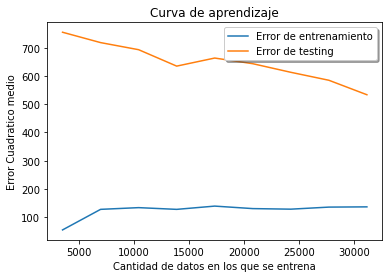
\includegraphics[width=0.6\textwidth]{curva_aprendizaje}
  \caption{Curva de aprendizaje del modelo final}
\end{figure}

\subsection{Análisis de los resultados obtenidos}

En el conjunto de entrenamiento hemos obtenido buenos resultados. Esto no nos sorprende por la alta capacidad de sobreajuste que tienen los árboles, a pesar de que hayamos fijado un par de parámetros como medida de regularización.

El error cuadrático medio en el conjunto de \emph{test} ha sido 4.12 veces mayor que en \emph{training}, mientras que en el error absoluto medio ha sido 1.79 veces mayor. El valor de $R^2$ en testing es de 0.55, lo cual indica unos resultados mediocres. Estamos explicando poco más de la mitad de la varianza en test con nuestro modelo.

A la vista de estos resultados, nos preguntamos si hemos tenido problemas de generalización a pesar de haber empleado un par de parámetros para regularizar. Se puede dar perfectamente el caso de que el modelo esté generalizando muy mal, o también de que el conjunto de \emph{test} sea complicado y cualquier modelo o medida de regularización provoque resultados peores a los que estamos obteniendo en test. Es por esto que vamos a emplear una serie de modelos como \emph{baselines} con los que comparar. Además, tenemos la sospecha de que esto pueda pasar por lo comentado en \emph{\ref{boxplot}. \nameref{boxplot}}.

Como \emph{baselines} vamos a emplear los siguientes modelos:

\begin{itemize}
    \item El segundo mejor modelo en el conjunto de datos al que solo aplicas borrado de \emph{outliers} (para poder realizar comparaciones justas que no dependan del conjunto de datos)
    \item Un regresor que siempre devuelve la mediia, usando \lstinline{DummyRegressor} de \lstinline{sklearn}
    \item Un regresor que siempre devuelve el valor cero, usando \lstinline{DummyRegressor}
\end{itemize}

Los resultados que se obtienen en test con estos regresores de referencia se muestran en la siguiente tabla:

\begin{table}[H]
  \centering
  \begin{tabular}{|c|c|c|c|}
  \hline
  \textbf{Modelos}  & \textbf{MSE} & \textbf{MAE} & \textbf{$R^2$} \\
  \hline
  MLP  & 1471.20  &  7.72 & -0.20 \\
  Dummy Media   & 1226.51 & 9.41 & 0.00 \\
  Dummy Cero & 1273.93 & 7.15 & -0.04 \\
  \hline
  \end{tabular}
  \caption{Resultados en test de los regresores de referencia}
\end{table}

Claramente en todos los modelos de referencia obtenemos resultados significativamente peores, y por tanto podemos concluir que, a pesar de nuestras dudas, el modelo considerado está aprendiendo de forma efectiva una función.

Nuestro modelo no está prediciendo de forma sistemática valores cercanos a la media ni valores constantemente cero, pues los resultados son mucho mejores que los que se obtienen siguiendo este comportamiento.

Cabe destacar que el \emph{baseline} \emph{MLP} obtiene un error cuadrático medio en training de 255.91, y por tanto, está teniendo problemas de generalización mucho más graves que el modelo que hemos considerado.

Notar que cuando obtenemos un valor de $R^2$ negativo, esto indica que nuestro modelo predice peor que el valor constantemente la media (por tanto \emph{Dummy} usando la media obtiene $R^2 = 0$).

Respecto a las curvas de aprendizaje, mantenemos el error en el conjunto de entrenamiento más o menos constante, gracias a la regularización que estamos aplicando. Mientras, el error en el conjunto de test desciende, y por tanto, estamos aprendiendo de forma efectiva la función. El error en \emph{testing} no alcanza una meseta ni tampoco un mínimo que no sea en el borde, así que es razonable pensar que con un conjunto de datos más grande podríamos mejorar el rendimiento de nuestro modelo.

La curva de aprendizaje del \emph{baseline} \emph{MLP} se muestra en la siguiente imagen:

\begin{figure}[H]
  \centering
  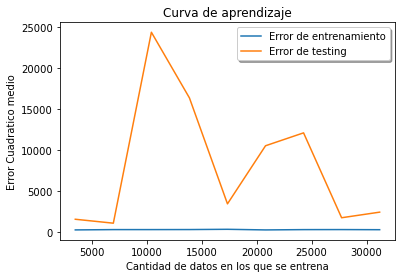
\includegraphics[width=0.6\textwidth]{curva_aprendizaje_mlp}
  \caption{Curva de aprendizaje del \emph{baseline} \emph{MLP}}
\end{figure}

En este caso, vemos como el modelo \emph{baseline} no está teniendo capacidad alguna de aprender la función objetivo.

Ahora, con la función \lstinline{where_did_the_model_failed} miramos los puntos en los que tenemos mayor error de salida, para tener una intuición de dónde falla más nuestro modelo. Nos interesa saber los valores de salida en los que más fallamos y el valor predicho para estos puntos. Las peores 25 etiquetas reales son: 1147,  896,  918,  704,  695,  507,  580,  564,  441,  434,  454,  455,  320,  409,   369,  527,  431,  284,  217,  338,   40,  229,  300,  306 y 253.

Ahora, mostramos un gráfico en el que en el eje $X$ mostramos el valor real de la etiqueta, y en el eje $Y$ mostramos el valor que nuestro modelo predice:

\begin{figure}[H]
  \centering
  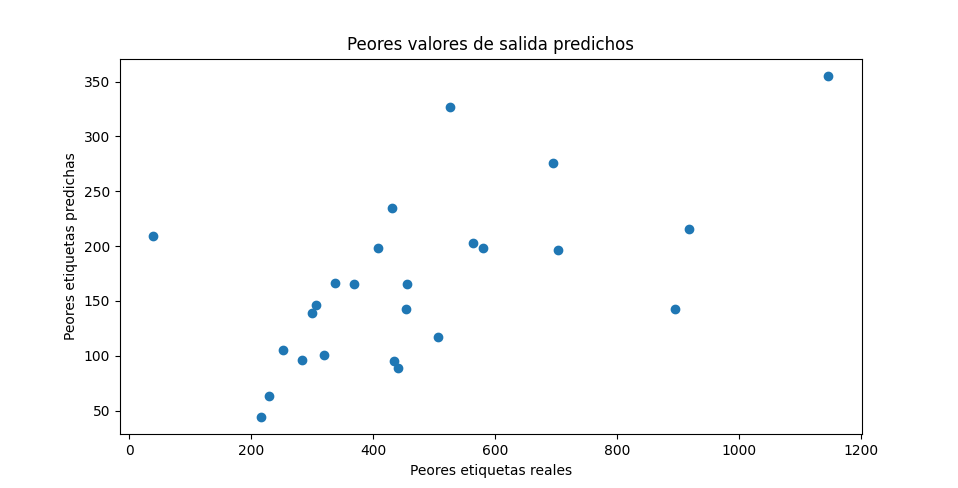
\includegraphics[width=\textwidth]{where_did_we_failed}
    \caption{Peores predicciones de nuestro modelo}
\end{figure}

Como podíamos suponer, como nuestra muestra de datos está muy concentrada en valores cercanos a cero de comentarios, la mayor parte de los ejemplos mal clasificados son aquellos con un número alto de comentarios (aquellos con más de 200 comentarios, cuando consideramos los 25 peores puntos). Esto podría mitigarse con el uso de un \emph{dataset} que tuviese más ejemplos de \emph{posts} con un número alto de comentarios.

Es significativo el punto con comentarios reales cercanos a cero que ha sido predicho con algo más de doscientos comentarios. Del mismo modo comentarios por encima de 800 comentarios se predicen a valores por debajo de 350 comentarios. Por tanto, nuestro modelo trabaja mal con valores extremadamente altos (por encima de 200 comentarios) tendiendo sus predicciones hacia valores más medios.

\textbf{En conclusión}, hemos encontrado un modelo robusto que ha funcionado bien teniendo en cuenta las particularidades y complicaciones que presentaba nuestro \emph{dataset}. Como mejoras al trabajo presentado podrían realizarse un procedimiento similar usando un \emph{dataset} con más representación de \emph{post} con muchos comentarios. También podría haberse presentado alguna técnica para sobrellevar este problema de representatividad, como \emph{data augmentation}, aunque no tenemos conocimiento de cómo aplicarla de forma eficiente y correcta.

\pagebreak
\section{Apéndice} \label{apendice}

\subsection{Características de la máquina}

\begin{lstlisting}
  Architecture:                    x86_64
  CPU op-mode(s):                  32-bit, 64-bit
  Byte Order:                      Little Endian
  Address sizes:                   39 bits physical, 48 bits virtual
  CPU(s):                          4
  On-line CPU(s) list:             0-3
  Thread(s) per core:              2
  Core(s) per socket:              2
  Socket(s):                       1
  NUMA node(s):                    1
  Vendor ID:                       GenuineIntel
  CPU family:                      6
  Model:                           142
  Model name:                      Intel(R) Core(TM) i7-7500U CPU @ 2.70GHz
  Stepping:                        9
  CPU MHz:                         2432.428
  CPU max MHz:                     3500,0000
  CPU min MHz:                     400,0000
  BogoMIPS:                        5802.42
  Virtualization:                  VT-x
  L1d cache:                       64 KiB
  L1i cache:                       64 KiB
  L2 cache:                        512 KiB
  L3 cache:                        4 MiB
  \end{lstlisting}

Además, la máquina tiene 8GB de memoria RAM.

\pagebreak
% Bibliografia
\bibliography{./References}
\bibliographystyle{ieeetr}

\end{document}
